% Copyright 2023  Ed Bueler

\documentclass[10pt,
               svgnames,
               hyperref={colorlinks,citecolor=DeepPink4,linkcolor=FireBrick,urlcolor=Maroon},
               usepdftitle=false]{beamer}

\mode<presentation>
{
  \usetheme{Madrid}

  \usecolortheme{beaver}

  \setbeamercovered{transparent}
  
  \setbeamerfont{frametitle}{size=\large}
}

\setbeamercolor*{block title}{bg=red!10}
\setbeamercolor*{block body}{bg=red!5}

\usepackage[english]{babel}
\usepackage[latin1]{inputenc}
\usepackage{times}
\usepackage[T1]{fontenc}
% Or whatever. Note that the encoding and the font should match. If T1
% does not look nice, try deleting the line with the fontenc.

\usepackage{empheq,bm,xspace,minted}
\usepackage{hyperref}

% If you wish to uncover everything in a step-wise fashion, uncomment
% the following command: 
%\beamerdefaultoverlayspecification{<+->}

\newcommand{\bb}{\mathbf{b}}
\newcommand{\bc}{\mathbf{c}}
\newcommand{\bbf}{\mathbf{f}}
\newcommand{\bl}{\bm{\ell}}
\newcommand{\br}{\mathbf{r}}
\newcommand{\bs}{\mathbf{s}}
\newcommand{\bx}{\mathbf{x}}
\newcommand{\by}{\mathbf{y}}
\newcommand{\bv}{\mathbf{v}}
\newcommand{\bu}{\mathbf{u}}
\newcommand{\bw}{\mathbf{w}}

\newcommand{\bzero}{\bm{0}}

\newcommand{\CC}{\mathbb{C}}
\newcommand{\RR}{\mathbb{R}}

\newcommand{\ddt}[1]{\ensuremath{\frac{\partial #1}{\partial t}}}
\newcommand{\ddx}[1]{\ensuremath{\frac{\partial #1}{\partial x}}}
\renewcommand{\t}[1]{\texttt{#1}}
\newcommand{\Matlab}{\textsc{Matlab}\xspace}
\newcommand{\Octave}{\textsc{Octave}\xspace}
\newcommand{\eps}{\epsilon}

\newcommand{\twovect}[4]{\ensuremath{{#1}_{#2} =
                            \begin{bmatrix} #3 \\ #4 \end{bmatrix}}}

\newcommand{\ftt}[1]{{\color{blue} \texttt{#1}}}

\newcommand{\optimaldef}{
\begin{definition}
an algorithm for computing a function on a class of problems, which acts on floating-point data of size $N$, is \emph{optimal} if it requires
   $$O(N) \qquad \text{ or } \qquad O(N\log N) \qquad \text{ flops}$$
\end{definition}
}


\title{Which linear systems can be solved optimally?}

\author{Ed Bueler}

\institute[]{UAF Math 692 Scalable Seminar}

\date{Spring 2023}


\begin{document}

\begin{frame}
  \maketitle
\end{frame}

\begin{frame}{Outline}
  \tableofcontents[hideallsubsections]
\end{frame}

\section{how fast is the basic matrix-vector product operation $z=Ax$?}

\newcommand{\bulletax}{\begin{bmatrix} \bullet \\ \bullet \\ \bullet \\ \bullet \end{bmatrix} = \begin{bmatrix} \bullet & \bullet & \bullet \\ \bullet & \bullet & \bullet \\ \bullet & \bullet & \bullet \\ \bullet & \bullet & \bullet \end{bmatrix} \begin{bmatrix} \bullet \\ \bullet \\ \bullet \end{bmatrix}}

\begin{frame}{matrix-vector products}
\begin{itemize}
\item the life-goal of a matrix $A \in \RR^{m\times n}$ is to act on (=multiply) vectors $x \in \RR^n$:
    $$z = Ax \qquad\quad \bulletax$$
\item this is a simple and familiar operation:
    $$z_i = \sum_{j=0}^{n-1} a_{ij} x_j \qquad \text{ for } i=0,\dots,m-1$$

    \begin{itemize}
    \item[$\circ$] note: I will index rows and columns starting from 0 in this talk
    \item[$\circ$] note: by default, vectors in $\RR^n$ are column vectors
    \end{itemize}
\item how fast is matrix-vector multiplication?
\item that is, what is its (\emph{algorithmic}) \emph{complexity}?
\end{itemize}
\end{frame}


\begin{frame}[fragile]
\frametitle{\texttt{matvec}}
\begin{itemize}
\item \phantom{actually,} this talk is based on genuine \phantom{pseudo}codes in Python\phantom{-ish}:
\end{itemize}
\begin{center}
\begin{minipage}{0.7\textwidth}
\begin{minted}[fontsize=\small]{python}
def matvec(A,x):
    from numpy import zeros, shape
    [m,n] = shape(A)
    z = zeros((m,1))
    for i in range(m):
        s = 0.0
        for j in range(n):
            s += A[i][j] * x[j]
        z[i] = s
    return z
\end{minted}
\end{minipage}
\end{center}
\end{frame}

\begin{frame}[fragile]
\frametitle{\texttt{matvec}}
\begin{itemize}
\item actually, this talk is based on genuine pseudocodes in Python-ish:
\end{itemize}
\begin{center}
\begin{minipage}{0.7\textwidth}
\begin{minted}[fontsize=\small]{python}
def matvec(A,x):
    for i = 0 to m-1:
        s = 0.0
        for j = 0 to n-1:
            s += A[i][j] * x[j]
        z[i] = s
    return z



\end{minted}
\end{minipage}
\end{center}
\end{frame}


\begin{frame}[fragile]
\frametitle{\texttt{matvec} flops}
\begin{center}
\begin{minipage}{0.7\textwidth}
\begin{minted}[fontsize=\small]{python}
def matvec(A,x):
    for i = 0 to m-1:
        s = 0.0
        for j = 0 to n-1:
            s += A[i][j] * x[j]
        z[i] = s
    return z
\end{minted}
\end{minipage}
\end{center}

\begin{itemize}
\item this \ftt{matvec} does exactly $2mn$ floating point operations (\emph{flops})
    \begin{itemize}
    \item[$\circ$] $n$ additions and $n$ multiplications for each of $m$ entries of result vector $Ax$
    \end{itemize}
\item complexity in big-O notation:
    \begin{itemize}
    \item[$\circ$] $O(mn)$ flops
    \item[$\circ$] $O(mn)$ storage (including inputs $A$ and $x$)
    \item[$\circ$] $O(mn)$ time (messy?)
    \end{itemize}
\end{itemize}
\end{frame}


\subsection{definition of ``optimal''}

\begin{frame}{my definition of \emph{optimal}}

\begin{itemize}
\item I will throw around ``optimal'' a lot in this talk
\end{itemize}

\optimaldef

\begin{itemize}
\item this means there exists $C$ so that for all problems, of any size $N$,
   $$(\text{flops}) \le C\, N \qquad \text{ or } \qquad (\text{flops}) \le C\, N\log N$$

    \begin{itemize}
    \item[$\circ$] quantifier order matters: \quad $\exists C \,\, \forall \text{ problems} \,\, \forall N \,\,  \dots$
    \end{itemize}
\item is \ftt{matvec} optimal?
\end{itemize}
\end{frame}


\begin{frame}{is \texttt{matvec} optimal?}

\hfill
{\scriptsize $\displaystyle \bulletax$}

\vspace{2mm}

\hfill
{\scriptsize $z = A x$} \hspace{17mm}

\vspace{-8mm}
\begin{itemize}
\item is \ftt{matvec} optimal?
\item it depends on what are the \alert{data} and the \alert{problems}!
\end{itemize}

\begin{enumerate}
\item<2->[1.] if the \alert{data $=$ vector $x$} ($N=n$), and we consider \alert{any matrix $A\in\RR^{m\times n}$ for which multiplication is valid}, then it \textbf{\emph{is not} optimal $O(N)$}
    \begin{itemize}
    \item[$\circ$] $2mn = 2m N \nleq C N$ for all problems \hfill $\gets$ \emph{$m$ depends on the problem}
    \end{itemize}
\item<3->[2.] if the \alert{data $=$ vector $x$} ($N=n$), and we consider a \alert{all matrices $A$ with (fixed) $m$ rows}, then it \textbf{\emph{is} optimal $O(N)$}, but the constant can be big
    \begin{itemize}
    \item[$\circ$] $2mn = 2m N \leq C N$ for $C=m$
    \end{itemize}
\item<4->[3.] if the \alert{data $=$ matrix $A$} ($N=mn$), and we consider \alert{any $x$}, then it \textbf{\emph{is} optimal $O(N)$}
    \begin{itemize}
    \item[$\circ$] $2mn = 2 N \leq C N$ for $C=2$
    \end{itemize}
\item<5>[4.] if the \alert{data $=$ vector $x$} ($N=n$), and we consider \alert{any tridiagonal matrix $A$}, then it \textbf{\emph{is} optimal $O(N)$}, assuming we don't do the zero multiplications
    \begin{itemize}
    \item[$\circ$] $2\cdot 3\cdot n = 6 N \leq C N$ for $C=6$
    \end{itemize}
\end{enumerate}
\end{frame}


\newcommand{\bulletaxtri}{\begin{bmatrix} \bullet \\ \bullet \\ \bullet \\ \bullet \end{bmatrix} = \begin{bmatrix} \bullet & \bullet & & \\ \bullet & \bullet & \bullet & \\ & \bullet & \bullet & \bullet \\ & & \bullet & \bullet \end{bmatrix} \begin{bmatrix} \bullet \\ \bullet \\ \bullet \\ \bullet \end{bmatrix}}

\begin{frame}[fragile]
\frametitle{tridiagonal matrix-vector product}

\begin{itemize}
\item to be honest, the tridiagonal case is a different algorithm:

\bigskip

\hfill
{\scriptsize $\displaystyle \bulletaxtri$}

\begin{center}
\begin{minipage}{0.8\textwidth}
\begin{minted}[fontsize=\small]{python}
def matvec_tri(A,x):
    z[0] = A[0][0] * x[0] + A[0][1] * x[1]
    for i = 1 to m-2:
        s = 0.0
        for j = i-1 to i+1:
            s += A[i][j] * x[j]
        z[i] = s
    z[m-1] = A[m-1][m-2] * x[m-2] + A[m-1][m-1] * x[m-1]
    return z
\end{minted}
\end{minipage}
\end{center}

\bigskip
\item this algorithm does $O(n)$ flops, so it is optimal in any interpretation
\end{itemize}
\end{frame}


\begin{frame}{regarding optimal algorithms}

\begin{itemize}
\item I will stick to my definition of ``optimal''!
\item however, it is fair to stop me and ask ``what is the data?'' or ``what is the class of problems?'' at any time
    \begin{itemize}
    \item[$\circ$] because whether an algorithm is optimal depends on an agreement regarding which is the data and which is the problem class
    \end{itemize}
\item<2-> it is fair to wonder if flops are a good metric for modern computers
    \begin{itemize}
    \item[$\circ$] but every other metric is messier?
\only<2>{
    \item[$\circ$] \emph{put up or shut up!}
}
\only<1,3>{
    \item[$\circ$] perhaps give a talk using another metric?
}
    \end{itemize}
\end{itemize}

\optimaldef
\end{frame}


\AtBeginSection[]
{
  \begin{frame}<beamer>
    \frametitle{Outline}
    \tableofcontents[currentsection,hideallsubsections]
  \end{frame}
}

\section{complexity of Gaussian elimination for linear systems $Ax=b$}

\begin{frame}{Gaussian elimination to solve linear systems $Ax=b$}

\begin{itemize}
\item Gaussian elimination (GE) with back-substitution (BS) is the familiar way to solve linear systems $Ax=b$ where $A\in\RR^{m\times m}$ is square
\item solving $Ax=b$ by GEBS is usually organized as $LU$ factorization (\emph{decomposition}) followed by triangular-system solves:
{\scriptsize
$$\begin{bmatrix} \bullet & \bullet & \bullet & \bullet \\ \bullet & \bullet & \bullet & \bullet \\ \bullet & \bullet & \bullet & \bullet \\ \bullet & \bullet & \bullet & \bullet \end{bmatrix}
=
\begin{bmatrix} \bullet & & & \\ \bullet & \bullet & & \\ \bullet & \bullet & \bullet & \\ \bullet & \bullet & \bullet & \bullet \end{bmatrix}
\begin{bmatrix} \bullet & \bullet & \bullet & \bullet \\ & \bullet & \bullet & \bullet \\ & & \bullet & \bullet \\ & & & \bullet \end{bmatrix}$$
}
$$A = L \, U \phantom{dflkja asdflk}$$
    $$Ax=b \quad \iff \quad
      \begin{matrix} A = LU \\
                     L(U x) = b \end{matrix} \quad \iff
      \begin{matrix} A = LU \\
                     U x = y \\
                     L y = b \end{matrix}$$

\vspace{-2mm}
   \begin{itemize}
   \item[$\circ$] this way of organizing does not affect the scaling
   \item[$\circ$] the triangular solves $Ux=y$ and $Ly=b$ each require exactly $m^2$ floating-point operations (\emph{exercise})
   \end{itemize}
\item partial pivoting should be done for numerical stability
   \begin{itemize}
   \item[$\circ$] this addition does not affect its scaling
   \end{itemize}
\end{itemize}
\end{frame}


\newcommand{\rbullet}{{\color{FireBrick} \bullet}}

\newcommand{\lubullets}{
$$\begin{bmatrix} \bullet & \bullet & \bullet & \bullet \\ \bullet & \bullet & \bullet & \bullet \\ \bullet & \bullet & \bullet & \bullet \\ \bullet & \bullet & \bullet & \bullet \end{bmatrix}
\to
\begin{bmatrix} \bullet & \bullet & \bullet & \bullet \\ 0 & \rbullet & \rbullet & \rbullet \\ 0 & \rbullet & \rbullet & \rbullet \\ 0 & \rbullet & \rbullet & \rbullet \end{bmatrix}
\to
\begin{bmatrix} \bullet & \bullet & \bullet & \bullet \\ 0 & \bullet & \bullet & \bullet \\ 0 & 0 & \rbullet & \rbullet \\ 0 & 0 & \rbullet & \rbullet \end{bmatrix}
\to
\begin{bmatrix} \bullet & \bullet & \bullet & \bullet \\ 0 & \bullet & \bullet & \bullet \\ 0 & 0 & \bullet & \bullet \\ 0 & 0 & 0 & \rbullet \end{bmatrix}$$
}

\begin{frame}[fragile]
\frametitle{LU decomposition pseudocode}

\begin{itemize}
\item the $A=LU$ step dominates the time for GEBS on $Ax=b$
\item as we convert $A$ to $U$ we zero-out columns below the diagonal
\item each column zeroing modifies a \alert{square of entries} to its right
\end{itemize}

\medskip
\begin{center}
\begin{minipage}{0.9\textwidth}
\begin{minted}[fontsize=\small]{python}
def lu(A):
    U, L = A, eye(m,m)
    for k = 0 to m-2:
        for i = k+1 to m-1:
            L[i][k] = U[i][k] / U[k][k]
            for j = k to m-1:
                U[i][j] = U[i][j] - L[i][k] * U[k][j]
    return U, L
\end{minted}
\end{minipage}
\end{center}

\bigskip
{\scriptsize
\lubullets
}
\end{frame}


\begin{frame}[fragile]
\frametitle{scaling of Gaussian elimination}

\begin{itemize}
\item $A=LU$ requires $\frac{2}{3} m^3 + O(m^2) = O(m^3)$ floating point operations
   \begin{itemize}
   \item[$\circ$] because the volume of an $m\times m\times m$ pyramid is $\frac{1}{3} m^3$
   \end{itemize}
\end{itemize}

\hfill 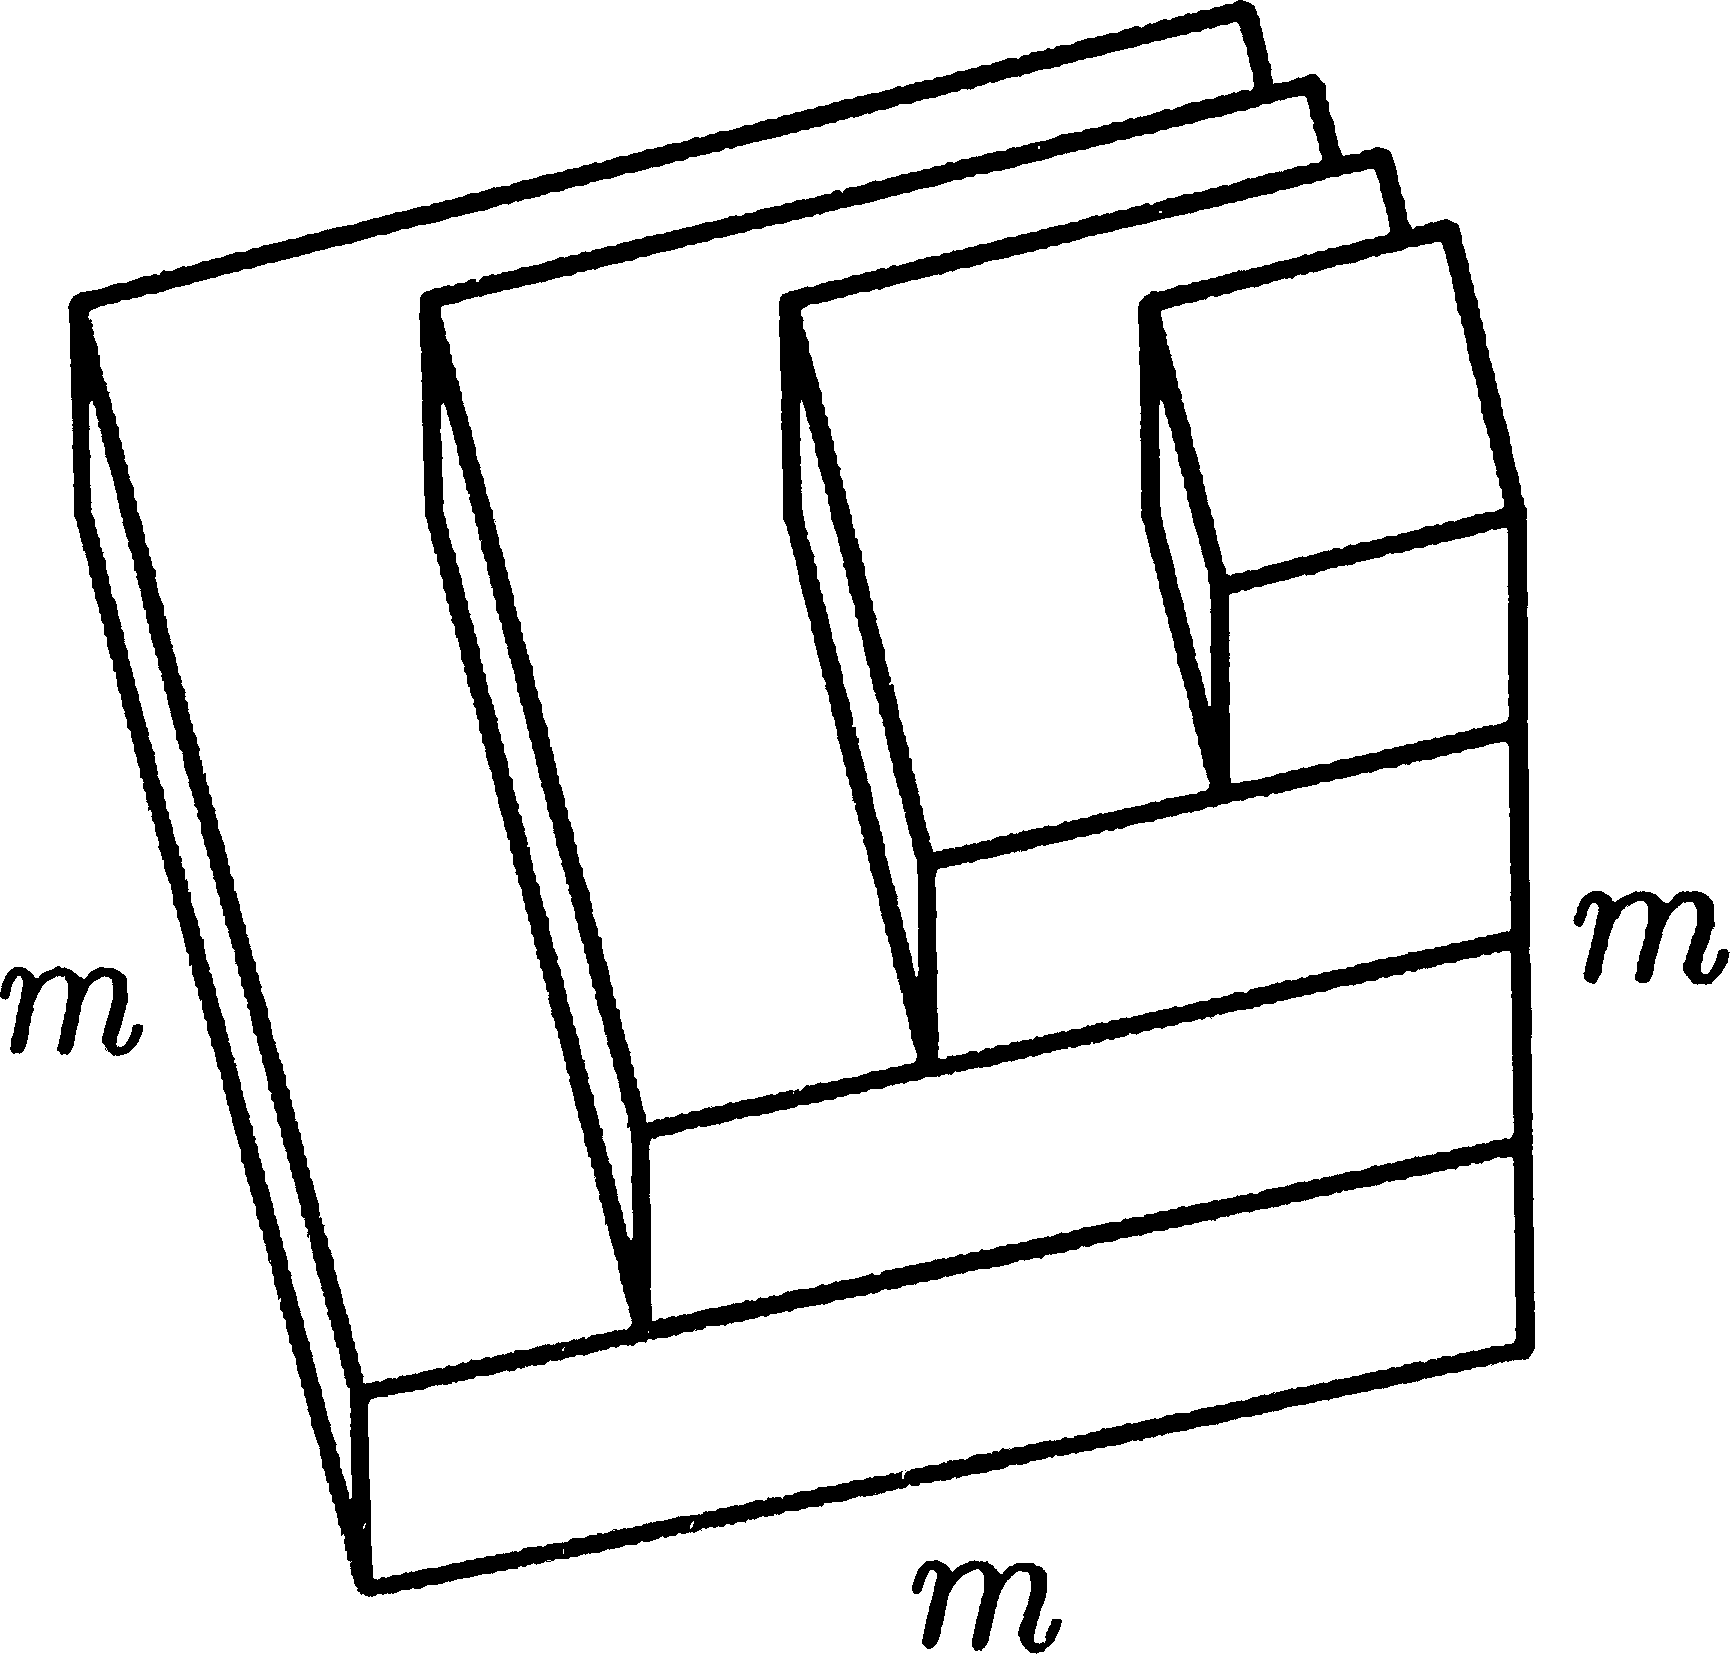
\includegraphics[width=0.2\textwidth]{images/gepyramid.png}

\vspace{-15mm}
\begin{minted}[fontsize=\footnotesize]{python}
def lu(A):
    U, L = A, eye(m,m)
    for k = 0 to m-2:
        for i = k+1 to m-1:
            L[i][k] = U[i][k] / U[k][k]
            for j = k to m-1:
                U[i][j] = U[i][j] - L[i][k] * U[k][j]
    return U, L
\end{minted}

\bigskip
{\scriptsize
\lubullets
}
\end{frame}


\begin{frame}{scaling for solving \textbf{dense} linear systems}

\begin{itemize}
\item the rest of the talk assumes $A$ is square and invertible
\item one may regard the data of ``solve $Ax=b$'' as the matrix $A\in\RR^{m\times m}$ itself
\item then an optimal solver for \textbf{dense} $A$ would require $O(m^2)$ flops
   \begin{itemize}
   \item[$\circ$] generic dense matrices $A$ have $m^2$ entries which affect the solution
   \item[$\circ$] touching each entry is $O(m^2)$
   \end{itemize}
\item GEBS is $O(m^3)$
\item $\exists$ solver algorithms for dense $A\in\RR^{m\times m}$ which scale as $O(m^{\,2.376})$
   \begin{itemize}
   \item[$\circ$] famously starting with V.~Strassen (1969). \emph{Gaussian elimination is not optimal}, Numer.~Math.~13, 354--356
   \item[$\circ$] these ``fast solvers'' can even be stable with respect to rounding errors? this is not clear to me! see J.~Demmel, I.~Dumitriu, O.~Holtz, and R.~Kleinberg (2007). \emph{Fast matrix multiplication is stable}, Numer.~Math.~106 (2), 199--224
   \end{itemize}
\item however, this ``fast dense solver'' game is not practical
   \begin{itemize}
   \item[$\circ$] fascinating algebra, but little impact on scientific/engineering software
   \item<2>[$\circ$] for the applications I care about, $O(m^{\,2.376})$ is catastophically slow
   \end{itemize}
\end{itemize}
\end{frame}


\begin{frame}{optimal solvers for $Ax=b$, arising from applications?}

\begin{itemize}
\item \alert{the rest of the talk assumes the size of the data is $m$}
   \begin{itemize}
   \item[$\circ$] $A\in\RR^{m\times m}$, $b \in \RR^m$
   \item[$\circ$] $m$ = (number of unknowns) = (number of rows in $A$) = (length of $b$)
   \end{itemize}
\item for special classes of $A\in\RR^{m\times m}$, are there optimal $O(m^1)$ solvers?
\item more precisely, are there special classes of matrices $A\in\RR^{m\times m}$, which routinely arise in applications, for which there are $O(m^1)$ solvers?
   \begin{itemize}
   \item[$\circ$] the answer will be ``yes''
   \end{itemize}
\item $O(m^1)$ solvers $\implies$ there \emph{must} be exploitable matrix structure
   \begin{itemize}
   \item[$\circ$] these are \emph{not} generic, dense matrices!
   \item[$\circ$] many are sparse
   \item[$\circ$] but some are dense!
   \end{itemize}
\item a \emph{huge} amount of science/engineering-relevant software supports these special matrix cases, and these optimal solver algorithms
\end{itemize}
\end{frame}


\section{tridiagonal and other banded matrices}

\begin{frame}{y}

\begin{itemize}
\item x
\end{itemize}
\end{frame}


\section{circulant matrices}

\begin{frame}{y}

\begin{itemize}
\item x
\end{itemize}
\end{frame}


\section{sparse storage}

\begin{frame}{y}

\begin{itemize}
\item x
\end{itemize}
\end{frame}


\section{paradigm: preconditioned Krylov iterations}

\begin{frame}{y}

\begin{itemize}
\item x
\end{itemize}

\hfill 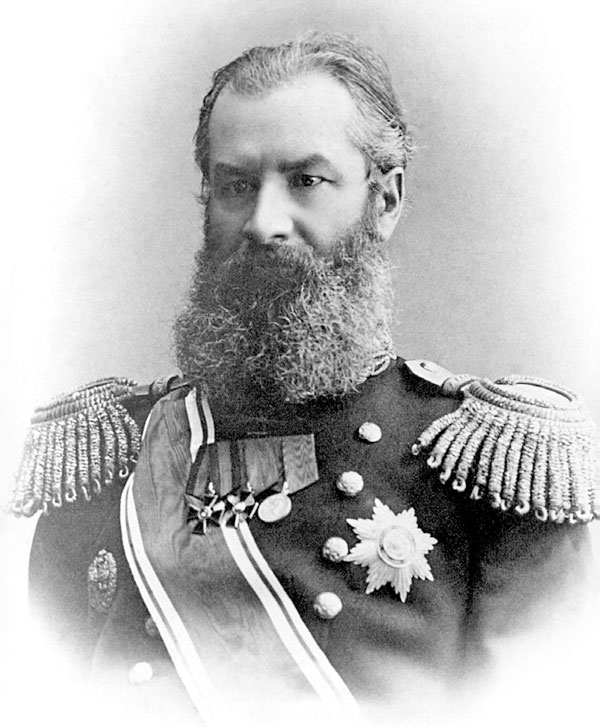
\includegraphics[width=0.2\textwidth]{images/akrylov.jpg}
\end{frame}


\section{multigrid: a teaser}

\begin{frame}{y}

\begin{itemize}
\item x
\end{itemize}
\end{frame}


\begin{frame}{references}

\begin{columns}
\begin{column}{0.85\textwidth}
\begin{itemize}
{\small
\item[] \textbf{A.~Brandt (1977)}. \emph{Multi-level adaptive solutions to boundary-value problems}, Mathematics of Computation 31 (138), 333--390
    \begin{itemize}
    \item[$\circ$] the guru of multigrid should be better known
    \end{itemize}
\item[] \textbf{W.~Briggs, V.~E.~Henson, \& S.~McCormick (2000)}.  \emph{A Multigrid Tutorial}, 2nd ed., SIAM Press, Philadelphia
\item[] \textbf{E.~Bueler (2021)}. \emph{PETSc for Partial Differential Equations}, SIAM Press, Philadelphia
    \begin{itemize}
    \item[$\circ$] optimal PDE solvers, multigrid, C and Python constructions
    \end{itemize}
\item[] \textbf{G.~Golub \& C.~van Loan (2013)}. \emph{Matrix Computations}, 4th ed., Johns Hopkins University Press, Baltimore
    \begin{itemize}
    \item[$\circ$] algorithms, banded \& circulant matrices, sparse storage
    \end{itemize}
\item[] \textbf{L.~Trefethen \& D.~Bau (2022)}. \emph{Numerical Linear Algebra}, 25th anniversary ed., SIAM Press, Philadelphia
    \begin{itemize}
    \item[$\circ$] clear thinking on linear systems
    \end{itemize}
\item[] \textbf{U.~Trottenberg, C.~Oosterlee, \& A. Schuller (2001)}.  \emph{Multigrid}, Elsevier, Oxford
}
\end{itemize}
\end{column}
\begin{column}{0.15\textwidth}
\hfill 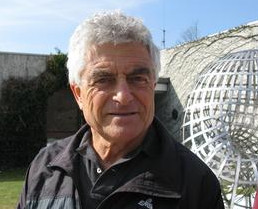
\includegraphics[width=\textwidth]{images/abrandt.jpg}

\vspace{7mm}
\hfill 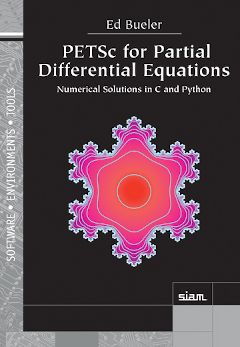
\includegraphics[width=0.8\textwidth]{images/bueler.jpg}

\bigskip
\hfill 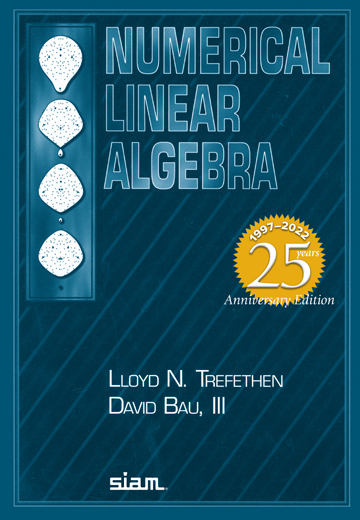
\includegraphics[width=0.8\textwidth]{images/trefethenbau.jpg}

\vspace{5mm}
\end{column}
\end{columns}
\end{frame}


\end{document}

